% !TEX root = ../main.tex
\newpage
% Раздел 1
\section{Анализ предметной области}\label{sec:razd1}
% анализ предметной области

\subsection{Обзор аналогичных программ}
\label{ssec:obzor}

% --------------------------------------------------
\subsubsection{GNU Privacy Guard}

% http://citforum.ru/security/cryptography/gnupg/

GNU Privacy Guard (GnuPG, GPG) -- программа для шифрования
информации и создания электронных цифровых подписей \cite{gnupg}.
GNU Privacy Guard является продуктом с открытым кодом, созданным
сообществом разработчиков.
Распространяется под лицензией General Public License (GPL).
Пакет изначально присутсвует в любом дистрибутиве Linux и
используется во многих приложениях.

Основные функции GnuPG:
\begin{itemize}
    \item Шифрование текста и файлов (используется несколько алгоритмов);
    \item Подписывание документов электронной цифровой подписью и проверка чужих подписей;
    \item Создание и управление списками открытых ключей респондентов.
\end{itemize}

Следует отметить, что GnuPG является утилитой, которая управляется только из
командной строки. Конечно, для упрощения работы с GPG существуют несколько
графических оболочек, а также множество компонент для разных языков.

В GnuPG используются разные криптографические алгоритмы: симметричные шифры,
шифрование с открытым ключом и смешанные алгоритмы.
Основной особенностью является система ключей. В GnuPG вы создаете себе несколько
ключей, причем каждый служит для отдельного действия (и использует разные
алгоритмы). Длина ключа может быть в пределах от 1024 до 4096 бит.

Для работы с документами доступны несколько команд:
\begin{itemize}
    \item Подписать документ;
    \item Зашифровать документ;
    \item Подписать и зашифровать документ;
    \item Проверить подпись.
\end{itemize}

Для шифрования файлов GnuPG использует не чистый алгоритм с открытым
ключом, а смешанный -- для документа формируется уникальный сеансовый ключ,
который шифруется шифром с открытым ключом, текст документа шифруется
симметричным шифром на основе сеансового ключа. Получатель с помощью своего
секретного ключа расшифровывает сначала сеансовый ключ, а потом с его помощью
сам документ. Такая схема работает быстрее, чем шифрование с открытым ключом,
а по надежности (криптостойкости) равна надежности самого слабого
из алгоритмов.

Теоретически, это позволяет упростить задачу дешифровки -- вместо взлома
системы шифрования с открытым ключом надо взломать только симметричный шифр,
то есть подобрать сеансовый ключ. Но такой метод даст возможность расшифровать
только одно сообщение, ведь для каждого документа сеансовый ключ генерируется
отдельно. Для симметричного шифрования по умолчанию применяется алгоритм CAST5.

GPG является многофункциональным инструментом для шифрования.
Он не дает возможности редактировать зашифрованные файлы без предварительной
расшифровки. Поэтому в дополнение к самому пакету необходимо иметь
оболочку, которая предоставляет такой функционал.

% --------------------------------------------------
% \newpage
\subsubsection{Vi/Vim}

% http://askubuntu.com/questions/436851/encrypting-text-editor
% https://github.com/vim/vim
% http://www.techrepublic.com/blog/it-security/vim-offers-strong-file-encryption-with-blowfish/

Vim -- улучшенная версия консольного текстового редактора Vi для
операционных систем семейства UNIX. Редактор имеет множество функций,
одной из которых является возможность работать с зашифрованными
текстовыми файлами. Для шифрования используется алгоритм Blowfish.

При создании файла можно указать флаг \texttt{-x}:

\begin{verbatim}
vim -x filename.txt
\end{verbatim}

После чего редактор просит пользователя ввести пароль:
\begin{verbatim}
Enter encryption key: *****
Enter same key again: *****
\end{verbatim}

Дальнейшая работа с зашифрованными файлами в редакторе vim ничем
не отличается от редактирования обычных текстовых файлов. Алгоритм
Blowfish является симметричным, поэтому при открытии файла необходимо
ввести тот же самый пароль.

Особенностью Vim является отсутствие необходимости сохранять
расшифрованную копию файла на жесткий диск перед его изменением.

% --------------------------------------------------
\newpage
\subsubsection{CryptoTE}

% http://askubuntu.com/questions/436851/encrypting-text-editor
% https://panthema.net/2009/cryptote/

CryptoTE -- текстовый редактор со встроенной функцией шифрования.
Данная программа позволяет создавать зашифрованные контейнеры,
которые могут содержать несколько файлов. Файлы могут быть как
текстовыми, так и бинарными (изображения, архивы и т. п.).

Программа позволяет редактировать текстовые файлы внутри контейнера
(рисунок \ref{fig:cryptote}), просматривать бинарные файлы
в шестнадцатиричном формате. Имеется возможность импортировать
и экспортировать файлы из контейнера.

CryptoTE по умолчанию использует симметричный алгоритм Serpent и
библиотеку zlib для сжатия данных. Имеется встроенный генератор
паролей.

\noindent
\begin{minipage}{\textwidth}
  \vspace{3.5mm}
  \centering
  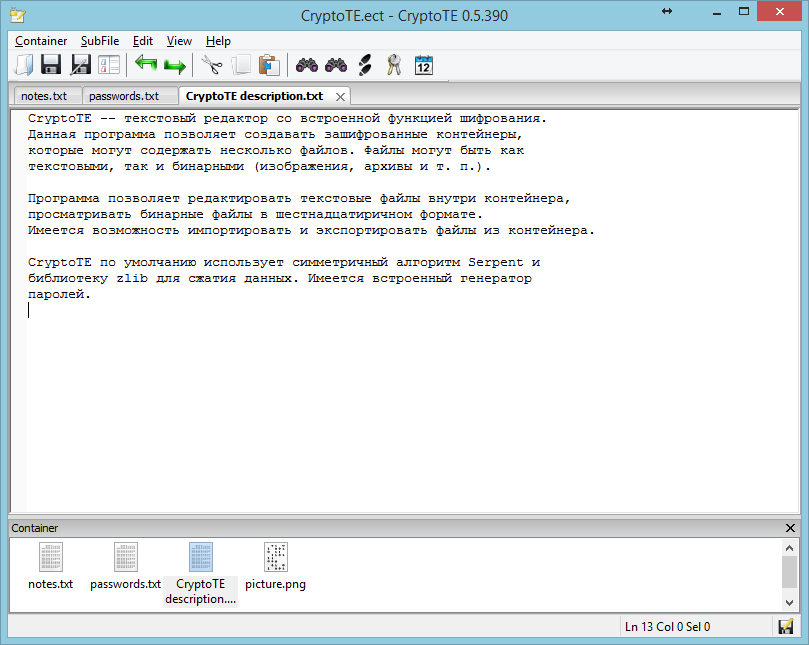
\includegraphics[scale=0.6]{./pics/cryptote-main.png}
  \captionof{figure}{Внешний вид редактора CryptoTE}\label{fig:cryptote}
  \vspace{3.5mm}
\end{minipage}

% --------------------------------------------------
\newpage
\subsubsection{KeyNote NF}

% http://jenyay.net/blog/2010/01/31/keynote-nf-eshhe-odin-outliner/

KeyNote NF -- структурный редактор (англ. outliner), позволяющий
структурированно хранить и редактировать заметки.

Файл с заметками может
содержать несколько вкладок, а каждая вкладка является
либо деревом заметок, либо одной заметкой с форматированием
(рисунок \ref{fig:keynotenf}). Сами заметки хранятся в формате
RTF (Rich Text Format). Программа позволяет шифровать файл
с заметками с помощью пароля.

\noindent
\begin{minipage}{\textwidth}
  \vspace{3.5mm}
  \centering
  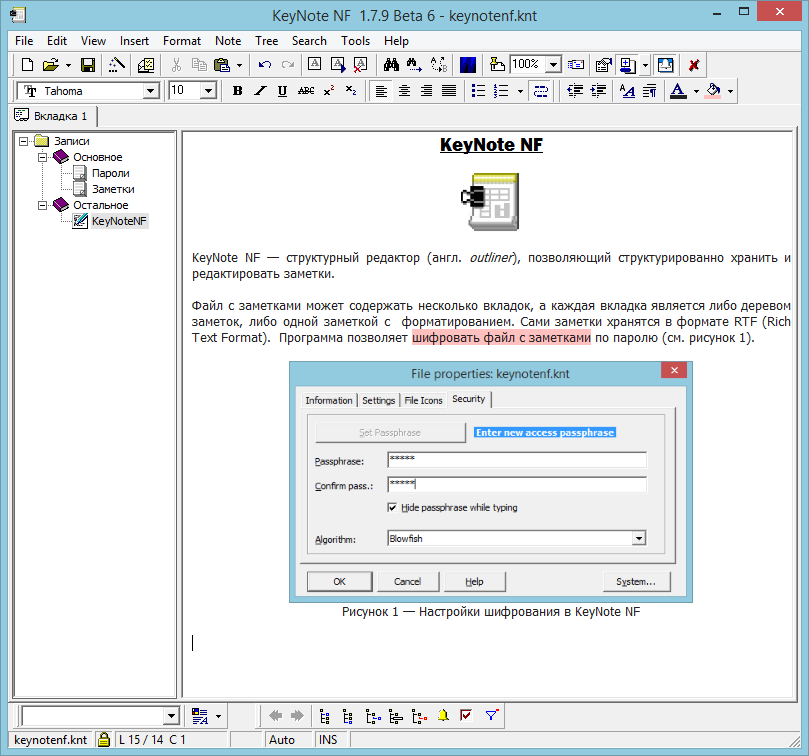
\includegraphics[scale=0.6]{./pics/keynote-main.png}
  \captionof{figure}{Внешний вид редактора KeyNote NF}\label{fig:keynotenf}
  \vspace{3.5mm}
\end{minipage}

% --------------------------------------------------
\newpage
\subsubsection{ProtectedText}

% https://www.protectedtext.com/
% https://play.google.com/store/apps/details?id=com.protectedtext.android

Приложение представляет из себя веб-сайт
\footnote{ProtectedText -- https://www.protectedtext.com/},
на котором любой пользователь имеет возможность бесплатно создать
одну или несколько страниц для хранения своих записей в текстовом
формате. Доступ к страницам осуществляется по паролю, который
вводит пользователь при первом сохранении текста на странице.
Страница может может содержать несколько вкладок
с текстовыми файлами (рисунок \ref{fig:protectedtext}).

По заверениям разработчиков, на сервере хранится только зашифрованный
текст и шифрование/дешифрование осуществляется на стороне пользователя.
С записками можно работать используя как персональный компьютер,
так и планшеты, смартфоны и остальные устройства с доступом в интернет.
При этом не требуется регистрация на сайте.

Стоит заметить, что пользователь может потерять доступ к своим записям
не только забыв пароль, но и потеряв ссылку на свою страницу с записями.

Пользователи устройств с ОС Anroid могут воспользоваться приложением
Safe Notes от разработчиков ProtectedText. Приложение позволяет создавать,
редактировать и шифровать заметки на мобильном устройстве, а так же
имеет возможность синхронизировать записи с ProtectedText.

\noindent
\begin{minipage}{\textwidth}
  \vspace{3.5mm}
  \centering
  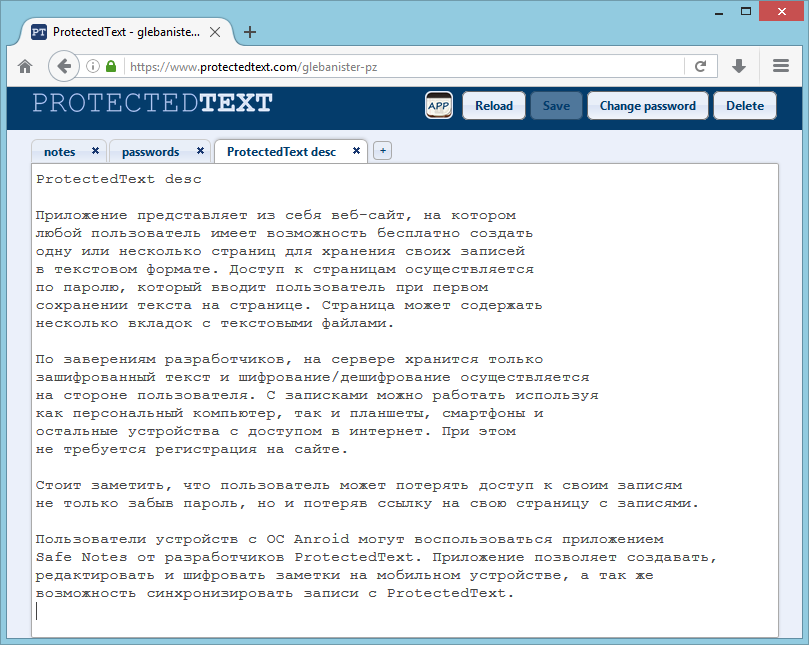
\includegraphics[scale=0.6]{./pics/protectedtext-main.png}
  \captionof{figure}{Внешний вид редактора ProtectedText}\label{fig:protectedtext}
  \vspace{3.5mm}
\end{minipage}

% --------------------------------------------------
\newpage
\subsubsection{NotepadCrypt}

% http://www.andromeda.com/people/ddyer/notepad/NotepadCrypt.html

NotepadCrypt -- простой текстовый редактор, основанный на Notepad2.
От Notepad2 редактор отличается наличием опции шифрования редактируемого
файла.

Приложение по умолчанию сохраняет текстовые файлы в незашифрованном виде.
Поэтому перед сохранением файла необходимо указать пароль, по которому
будет производиться шифрование (рисунок \ref{fig:notepadcrypt}).
Программа использует алгоритм шифрования AES-256.

Также стоит отметить возможность указать мастер-пароль (англ. master passphrase).
Файлы сохраненные с указанным мастер-паролем могут быть восстановлены
в случае утери пароля от зашифрованного файла.

\noindent
\begin{minipage}{\textwidth}
  \vspace{3.5mm}
  \centering
  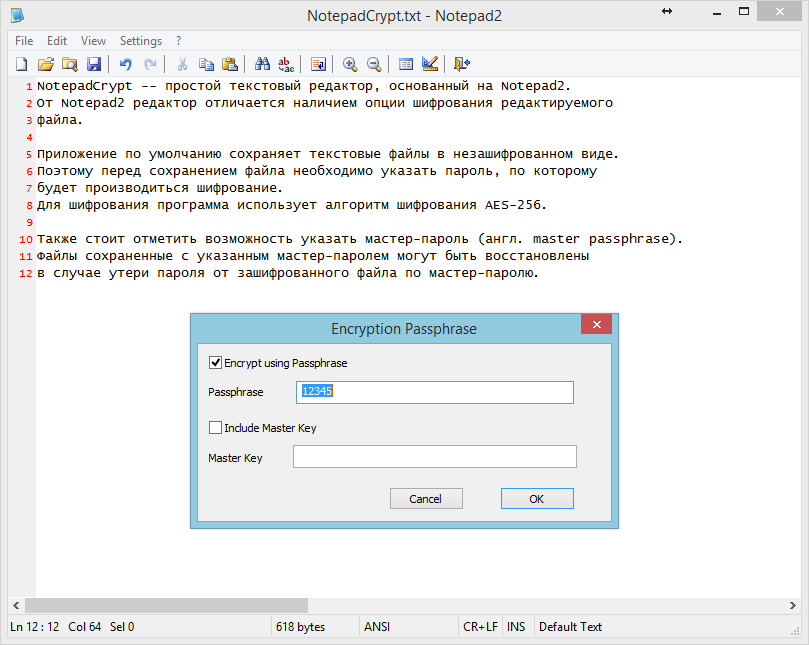
\includegraphics[scale=0.6]{./pics/notepadcrypt-main.png}
  \captionof{figure}{Внешний вид редактора NotepadCrypt}\label{fig:notepadcrypt}
  \vspace{3.5mm}
\end{minipage}

% --------------------------------------------------
\newpage
\subsubsection{Notepad++ (с аддоном NppCrypt)}

Notepad++ -- текстовый редактор, позволяющий расширить свой функционал
с помощью плагинов. Одним из интересных плагинов является NppCrypt.
Плагин дает возможность пользователю зашифровать текст.

В отличие от описаных ранее редакторов, плагин лишь изменяет выделенный
текст внутри редактора. Таким образом перед сохранением отредактированного
текста пользователю необходимо его зашифровать, выбрав соответствующую опцию
в меню доступа к функциям плагина NppCrypt (рисунок \ref{fig:notepadpp}).
Аналогично после открытия зашифрованного файла необходимо выполнить
дешифрование, после чего можно приступить к редактированию текста.
Такая работа с файлом не слишком удобна и существенно снижает
эффективность пользователя.

В то же время плагин имеет довольно гибкие настройки и множество опций
симметричного шифрования. Шифротекст может храниться в бинарном,
в шестнадцатиричном виде или в кодировке base64. Текст можно зашифровать
одним из множества алгоритмов (IDEA, CAST5, Blowfish, AES-256 и т. д.).
Плагин позволяет выбрать один из нескольких режимов
шифрования (ECB, CBC, CFB, OFB и т. д.). Также имеются настройки
алгоритма генерации ключа по паролю.

\noindent
\begin{minipage}{\textwidth}
  \vspace{3.5mm}
  \centering
  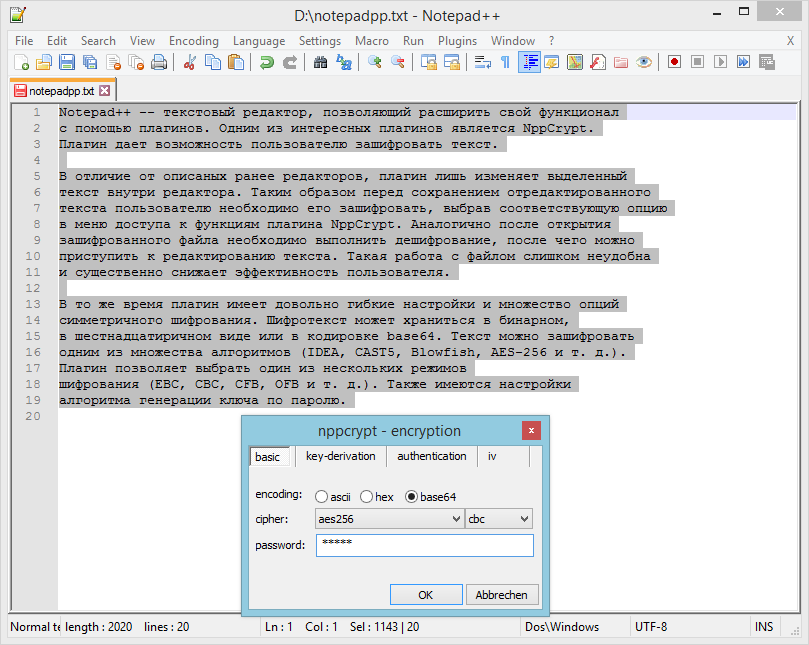
\includegraphics[scale=0.6]{./pics/notepadpp-main.png}
  \captionof{figure}{Внешний вид редактора Notepad++}\label{fig:notepadpp}
  \vspace{3.5mm}
\end{minipage}

% % --------------------------------------------------
% \subsubsection{Bitmask}
%
% Bitmask -- приложение с открытым исходным кодом, обеспечивающее легкую в
% использовании и безопасную зашифрованную коммуникацию.
% Bitmask предоставляет сервис для шифровании электронной почты, которая
% в то же время обратно совместима с существующим протоколом OpenPGP для
% безопасной электронной почты.
%
% В число особенностей программы входят:
% \begin{itemize}
%     \item Полное сквозное шифрование. Всякий раз, когда это возможно, все
%     сообщения шифруются непрерыно на клиентском устройстве.
%     \item Безопасное хранение. Все входящие сообщения автоматически шифруются,
%     потому только вы можете прочесть их (в том числе мета-данные).
%     \item Автоматическое управление ключами. Пользователю не нужно
%     беспокоиться о генерации, обнаружении или проверке ключей.
% \end{itemize}
%
% \subsubsection{opmsg}
%
% % https://github.com/stealth/opmsg
%
% Opmsg является альтернативой GPG для шифрования и подписания почтовых сообщений.
% Программа распространяется под лицензией GPLv3.


\newpage
\subsection{Сравнительный анализ}

В таблице \ref{tab:sravn} приведен сравнительный анализ описанных
в пункте \ref{ssec:obzor} программных средств для шифрования
текстовых документов.

\noindent
\begin{minipage}{\textwidth}
  \vspace{3.5mm}
  \captionof{table}{Сравнение приложений для шифрования текстовых записей}
  \vspace{-3.5mm}
  \label{tab:sravn}
  \footnotesize
  \begin{tabular}{|L{25mm}|L{30mm}|L{30mm}|L{40mm}|C{25mm}|}
    \hline
    Название &
      Лицензия &
      %Открытость кода &
      Операционная система &
      Криптографические методы &
    Графический интерфейс \\\hline

    GNU Privacy Guard &
      GNU GPLv3 &
      %Код открыт &
      Linux, Windows, Mac OS X &
      AES, DES, Blowfish, CAST5, MD5, SHA1, SHA256, SHA512, RSA, ... &
      $-$
    \\\hline

    Vim  &
      GPL-совместимая &
      %Код открыт &
      Linux, Windows, OS X &
      Blowfish &
      $-$
    \\\hline


    CryptoTE &
      GNU GPLv2 &
      %Код открыт &
      Linux, Windows &
      Serpent &
      $+$
    \\\hline

    KeyNote NF &
      MPLv2.0 &
      %Код открыт &
      Windows &
      Blowfish, IDEA &
      $+$
    \\\hline


    ProtectedText &
      \makebox[30mm][c]{$-$} &
      %Частично открыт &
      Веб-приложение &
      AES, SHA256 &
      $+$
    \\\hline

    NotepadCrypt &
      GNU GPLv3 &
      %Код открыт &
      Windows &
      AES, SHA256 &
      $+$
    \\\hline

    Notepad++ (NppCrypt) &
      GNU GPLv3 &
      %Код открыт &
      Linux, Windows &
      AES, DES, CAST5, IDEA, Blowfish,
      MD5, SHA1, SHA256, SHA512, ... &
      $+$
    \\\hline
  \end{tabular}
  \vspace{3.5mm}
\end{minipage}

\subsection{Постановка задачи}
Хранение и быстрый доступ к конфиденциальной информации -- важная
необходимость в жизни современного человека. Сравнительный анализ показал, что
актуально и целесообразно спроектировать и реализовать программный продукт
в соответствии со следующими требованиями:
\begin{itemize}
    \item Наличие графического интерфейса;
    \item Работа с зашифрованными файлами с использованием прозрачного шифрования;
    \item Использование различных алгоритмов шифрования;
    \item Мультиплатформенность.
\end{itemize}
